 

\documentclass[xcolor={dvipsnames}]{beamer}
\usepackage{amsmath}
% \usepackage{beamerthemesplit} // Activate for custom appearance
\usepackage{hyperref}
\usepackage{ragged2e}

\title{Ensemble Methods (Part II)\\
Gradient Boosting}
\author{Schwartz}
\date{\today}

\begin{document}

\frame{\titlepage}

\frame
{
 \frametitle{The most powerful prediction algorithm on the planet}

{
\fontfamily{<familyname>}\selectfont
\begin{quote}
\tiny
\justify

In ``The BellKor Solution to the Netflix Grand Prize''
Yehuda Koren reported on the use of gradient boosted decision trees (GBDT) in the top performing algorithm.  
The Netflix Prize was an open competition for the best collaborative filtering algorithm to predict user ratings for films. The competition was open to anyone not connected with Netflix or a resident of Cuba, Iran, Syria, North Korea, Myanmar or Sudan. On 21 September 2009, the grand prize of \$1,000,000 was given to the Pragmatic Chaos team which bested Netflix's own prediction algorithm by 10.06\%.    ``The Ensemble''  tied  the best score 19 minutes and 56 seconds later but got nothing. 
BellKor's solution hasn't been used in production as it is ``too complicated''.  
Today gradient boosting (usually in the form of XGBoost) satisfies itself with being the winningest algorithm in  
much smaller challenges such as Kaggle competitons.
\end{quote}
}

\begin{figure}
\centering
\fbox{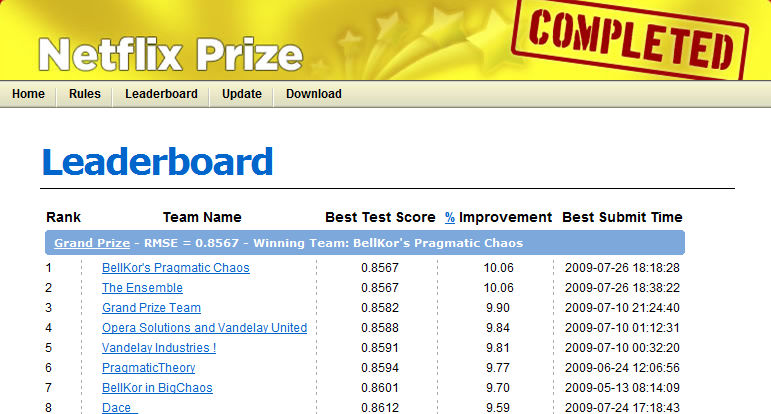
\includegraphics[width=3.65in]{stuff/NetflixPrize.png}}
\end{figure}
}


\frame
{
 \frametitle{Objectives}

\begin{itemize}
\item Understand gradient boosting   
\begin{itemize}
\item<2-> as a basic, simple, general algorithm  
\item<3-> as an ensemble of sequential ``weak learners''
\item<4-> as a series of regressions on sequential residuals
\item<5-> as a general gradient descent algorithm  
\item<6-> in it's earliest/latest incarnation as AdaBoost/XGBoost
\item[]
\end{itemize}
\item<7-> Understand the tuning parameters of tree-based boosting
\begin{itemize}
\item<8-> Distinguish tree parameters versus boosting parameters 
\item<9-> Understand implementation/tuning via grid search 
\item[]
\end{itemize}
%\item<10-> Understand partial dependency plots
\item<10-> \emph{Critique} and \emph{Sell} gradient boosting 
\begin{itemize}
\item<11-> As compared to other ensemble methods
\end{itemize}
\end{itemize}

}


\frame
{
 \frametitle{Sequential ``weak learners''}

\begin{enumerate}
\item<1-> Student 1 takes exam
\item<2-> Student 2 takes exam \emph{knowing how student 1 did}
\item[$\vdots$]<3-> 
\item[$k$]<3-> Student $k$ takes exam \emph{knowing how student $k-1$ did}
\item[$\vdots$]<4-> 
\item[$n$]<4-> Student $n$ takes exam \emph{knowing how student $n-1$ did}
\item[]<4-> 
\end{enumerate}

\begin{itemize}
\item<5-> \emph{Sequential learners} focus effort on outcomes predicted poorly 
\underline{by previous learners} as opposed to those predicted accurately 
\item[]
\item<6-> \emph{Weak learners} consistently predict outcomes but with  accuracy \underline{only $\epsilon$ slightly better than chance} \textcolor{gray}{(so high bias/low variance)}   
\end{itemize}

\begin{figure}
\centering
\onslide<7->{
Can many \emph{sequential weak learners} \\be used to make a powerful prediction tool?}

\onslide<8->{\textcolor{gray}{Do you think such an approach could suffer from overfitting?}}
\end{figure}
}


\frame
{
 \frametitle{Sequential Estimators Notation}

\begin{itemize}
\item Let $W$ be an untrained weak learner and $f_k({\boldsymbol x})$ be 
an estimator that predicts outcome $Y$ based on features ${\boldsymbol x}$ 
\item[]
\item[] Define a new estimator  
$$f_{k+1}({\boldsymbol x}) = f_k({\boldsymbol x}) + \alpha_k W({\boldsymbol x}, \gamma_k)$$ 
where $W$ is trained on ${\boldsymbol x}$ ``in the 
presence of'' $f_k({\boldsymbol x})$

\item[]
\item<2-> E.g., let $W$ be a tree and $\gamma_k = \text{number of splits} = 1$
\item<3->[] So $W$ is a stump -- a weak learner$^*$
\item<4-> $W$ is fit to \emph{improve} the available prediction of $Y$ from $f_k({\boldsymbol x})$  
\item<5-> But the negligible impact of $W^*$ will be further muted by $\alpha_k$
\item<5-> \textbf{$\alpha_k$ controls the \textcolor{red}{\underline{learning rate}} of the boosting algorithm}
\end{itemize}
}



\frame
{
 \frametitle{Compare and Contrast}
\LARGE
\begin{itemize}
\item[(A)] \textcolor{pink}{Tree} \onslide<2->{\small $\hat f^{(1)}({\boldsymbol x})$}
\LARGE %Sepia
\item[(B)] \textcolor{Dandelion}{Bagging} \onslide<2->{\small $\frac{1}{m} \sum \hat f^{(k)}({\boldsymbol x})$} 
\LARGE
\item[(C)] \textcolor{SkyBlue}{Random Forests} \onslide<2->{\small $\frac{1}{m} \sum \hat f^{(k)}({\boldsymbol x}),$ \text{ with small Cor$[\hat f^{(k)}, \hat f^{(k')}]$}}
\LARGE
\item[(D)] \textcolor{ForestGreen}{Sequential Weak Learners} \onslide<2->{\scriptsize$\sum \alpha_k\hat W_k({\boldsymbol x}, \gamma_k| \hat W_{k-1}, \cdots \hat W_{1})$}
\end{itemize}

\begin{figure}
\centering
\onslide<3->{
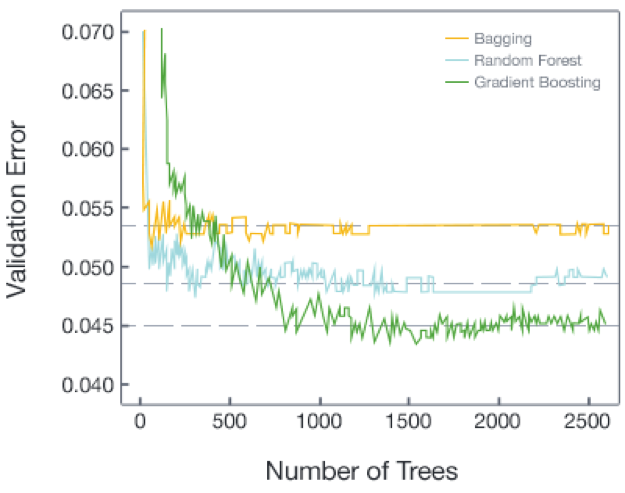
\includegraphics[width=2.5in]{stuff/number-of-trees.png}}
\end{figure}

}


\frame
{
 \frametitle{Gradient Boosting \emph{Tuning}}
\begin{itemize}
\item[] \underline{Gradient Boosting is typically applied using trees} 
\item<2-> \textcolor{SkyBlue}{Shallow trees (stumps?) provide weak learners/reduce tuning}
\item<3-> \textcolor{SkyBlue}{Nonetheless, number of leaves, depth, minimum split size, minimum leaf, size, and restricted features$^*$ can be tuned...} 
\item<4-> \textcolor{CornflowerBlue}{The learning rate/number of trees ($\alpha/m$) needs to be tuned}
\item<5-> \textcolor{SeaGreen}{Stochastic Gradient Boosting using subsamples also available}
\item<6-> \textcolor{red}{Careful parameter tuning is necessary for good performance}\\${}$\\
\end{itemize}
\begin{figure}
\centering
\vspace{-.75in}
\onslide<3>{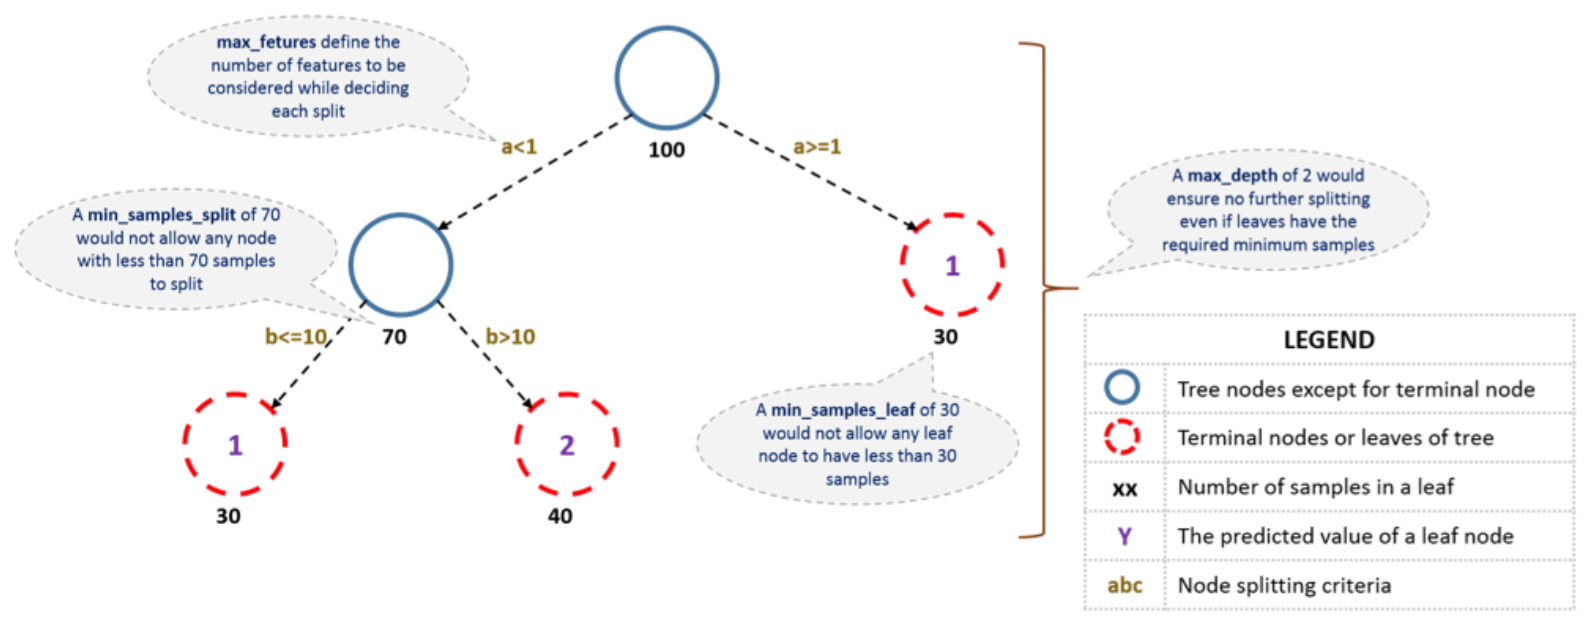
\includegraphics[width=4.5in]{stuff/tunes.png}}

\vspace{-1.75in}
\onslide<4>{\fbox{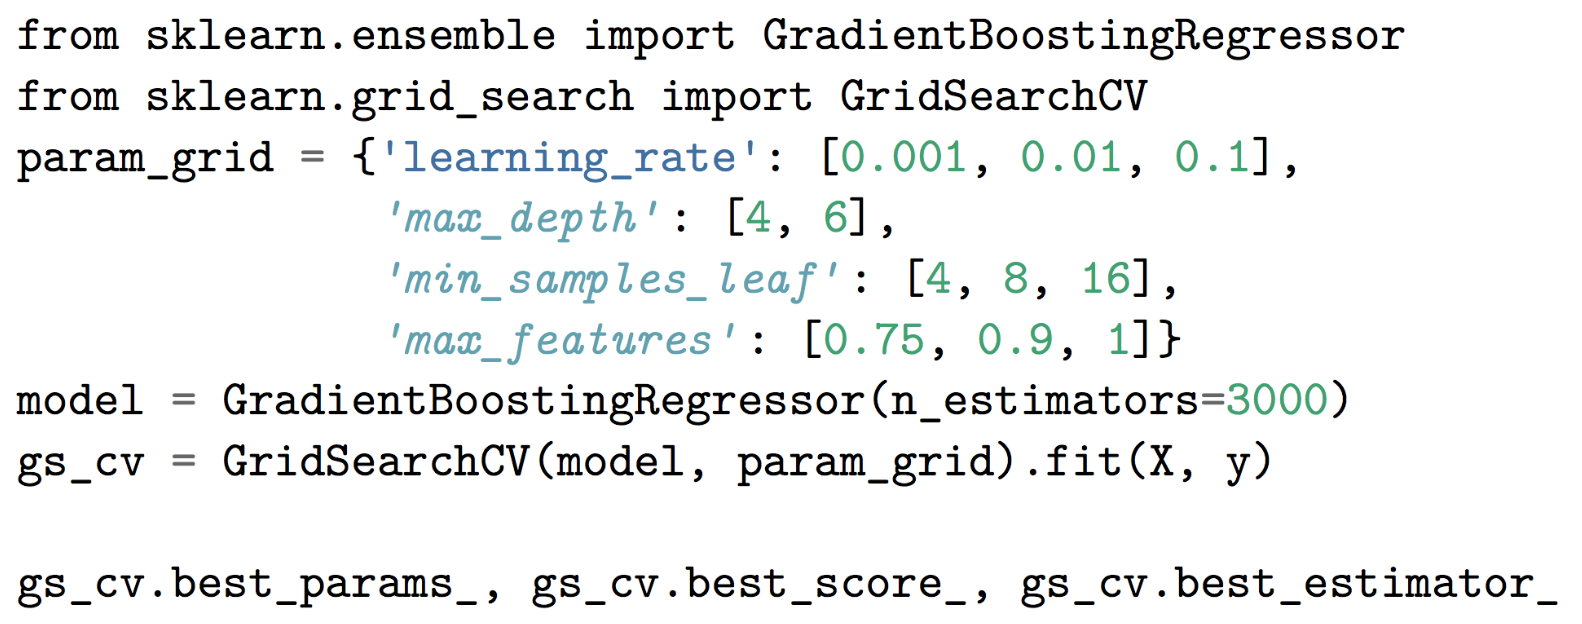
\includegraphics[width=4in]{stuff/grid1.png}}}

\vspace{-1.5in}
\onslide<5->{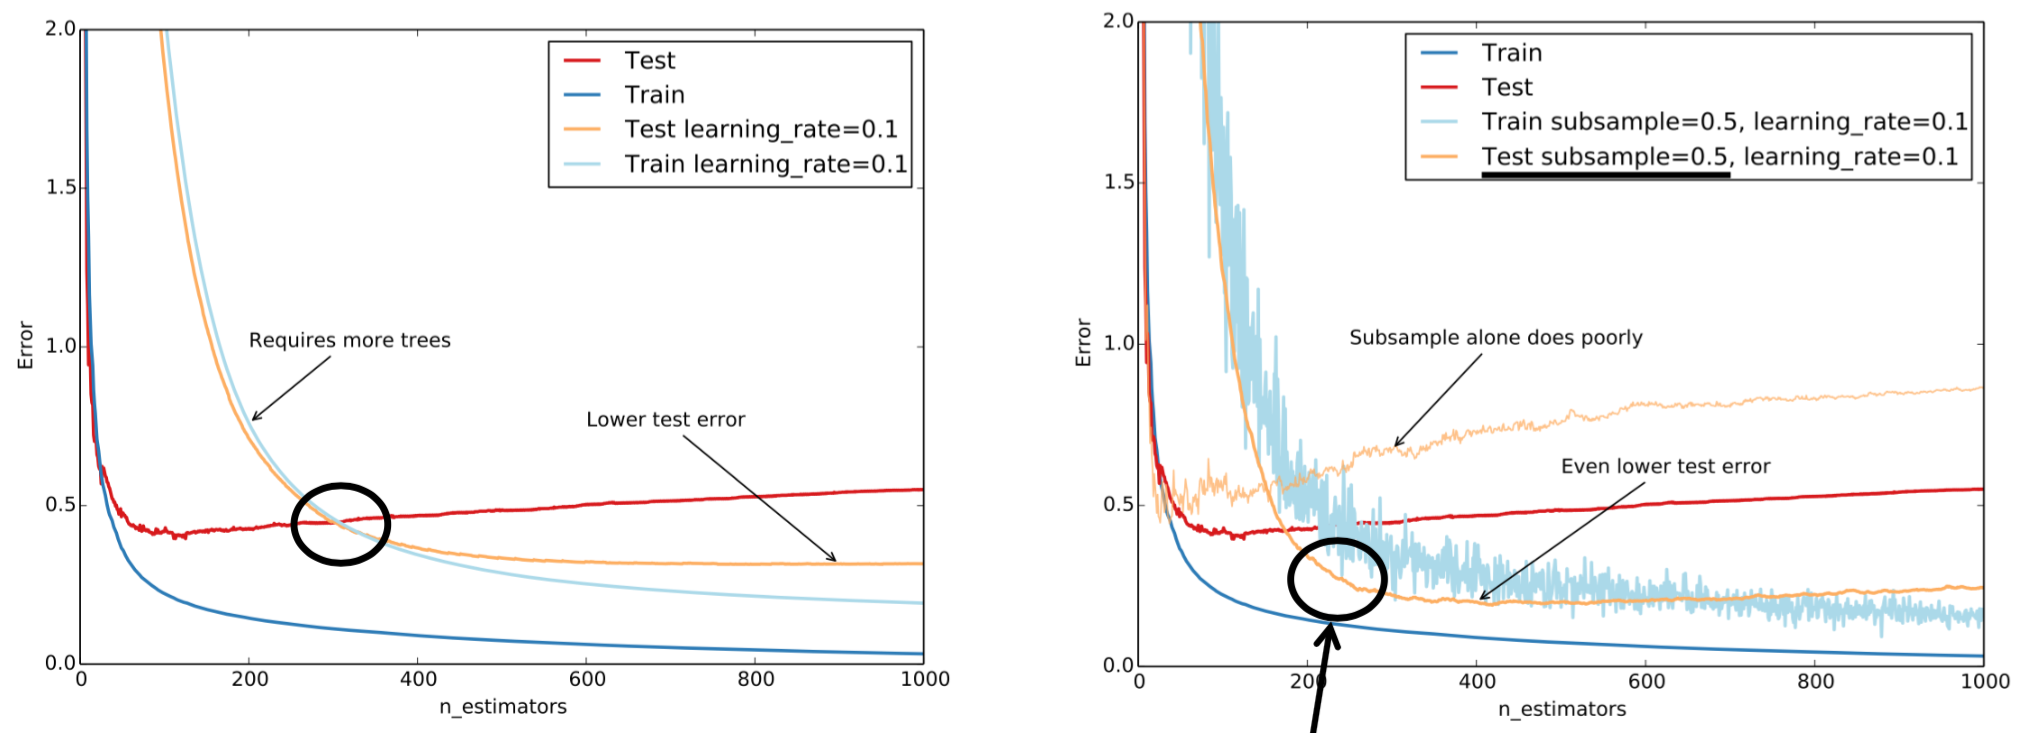
\includegraphics[width=4.2in]{stuff/subsample.png}}

\end{figure}
}

\frame
{
 \frametitle{Buy or Sell Gradient Boosting?}

\begin{itemize}
\item<1-> Pros
\begin{itemize}
\item<2-> Netflix Prize \& Kaggle Competitions
\end{itemize}
\item<1-> Cons
\begin{itemize}
\item<3-> Extensive tuning required
\item<4->[] Unlike Bagging/Random Forests, increasing the number of trees used for Boosting  \emph{CAN CAUSE} overfitting 
\item<5-> Inherently non-parallelizable 
\end{itemize}
\item[]
\item[] 
\item[]
\item[]<6-> Why does this work better than Random Forests, etc.?
\end{itemize}


}




\frame
{
 \frametitle{Fitting regressions on sequential residuals}

\begin{columns}
\begin{column}{.3\textwidth}

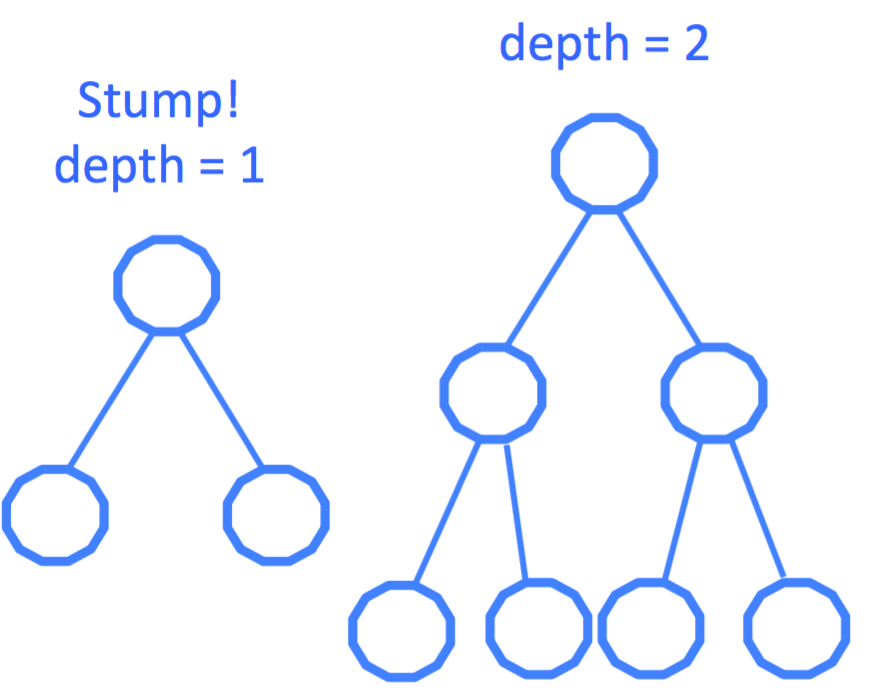
\includegraphics[width=1.5in]{stuff/stump.png}

\end{column}
\begin{column}{.75\textwidth}

\footnotesize
 \begin{enumerate}
 \item<2-> Set $\hat f^{(0)}({\boldsymbol x}_i)=0$ and  $\hat \epsilon^{(1)}_i = Y_i$

 \item<3-> For $k = 1, \cdots m$ \\ 
 \begin{enumerate}
\footnotesize
\item<4-> Fit a tree $\hat f^{(k)}$ to $\hat {\boldsymbol \epsilon}^{(k)}$ using features ${\boldsymbol x}$
\item<5-> Update the estimator $\hat f^{(k+1)} = f^{(k)} + \alpha_k f^{(k-1)}$
\item<6-> Update the residuals $\hat \epsilon^{(k+1)}_i = \hat \epsilon^{(k)}_i -  \alpha_k f^{(k)}({\boldsymbol x}_i)$
\end{enumerate}
\item<7-> Return the boosted model $\hat f({\boldsymbol x}_i) = \sum_{k=1}^m \alpha_k f^{(k)}({\boldsymbol x}_i)$ 
\end{enumerate}

\end{column}
\end{columns}


\begin{figure}
\centering
\hspace*{-.35in}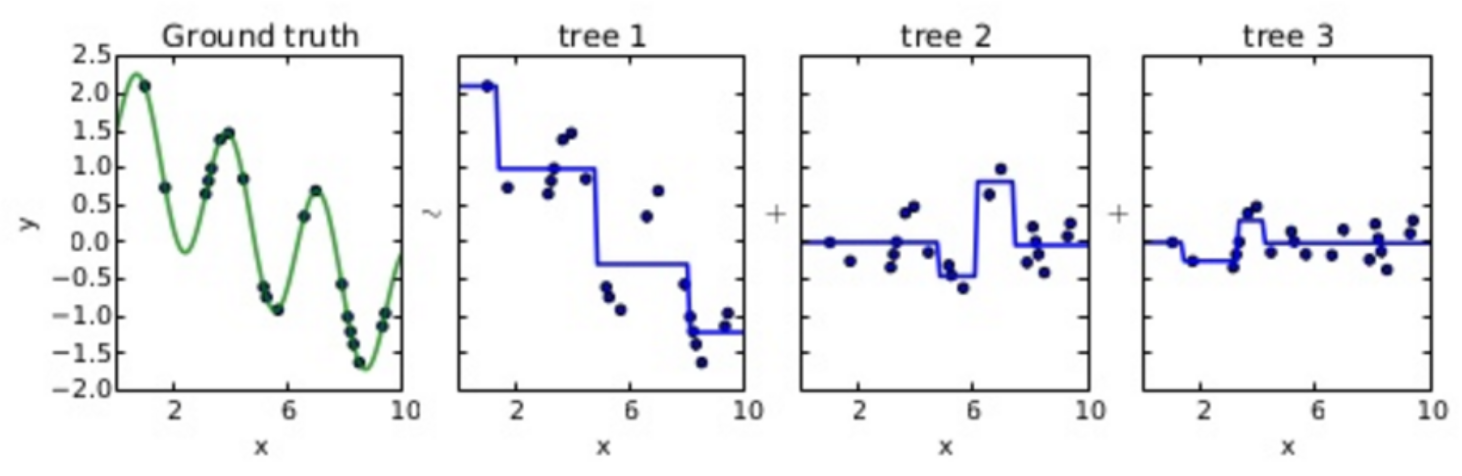
\includegraphics[width=4.85in]{stuff/residualsgradient.png}
\end{figure}

}




\frame
{
 \frametitle{Fitting regressions on sequential residuals}

\begin{figure}
\centering
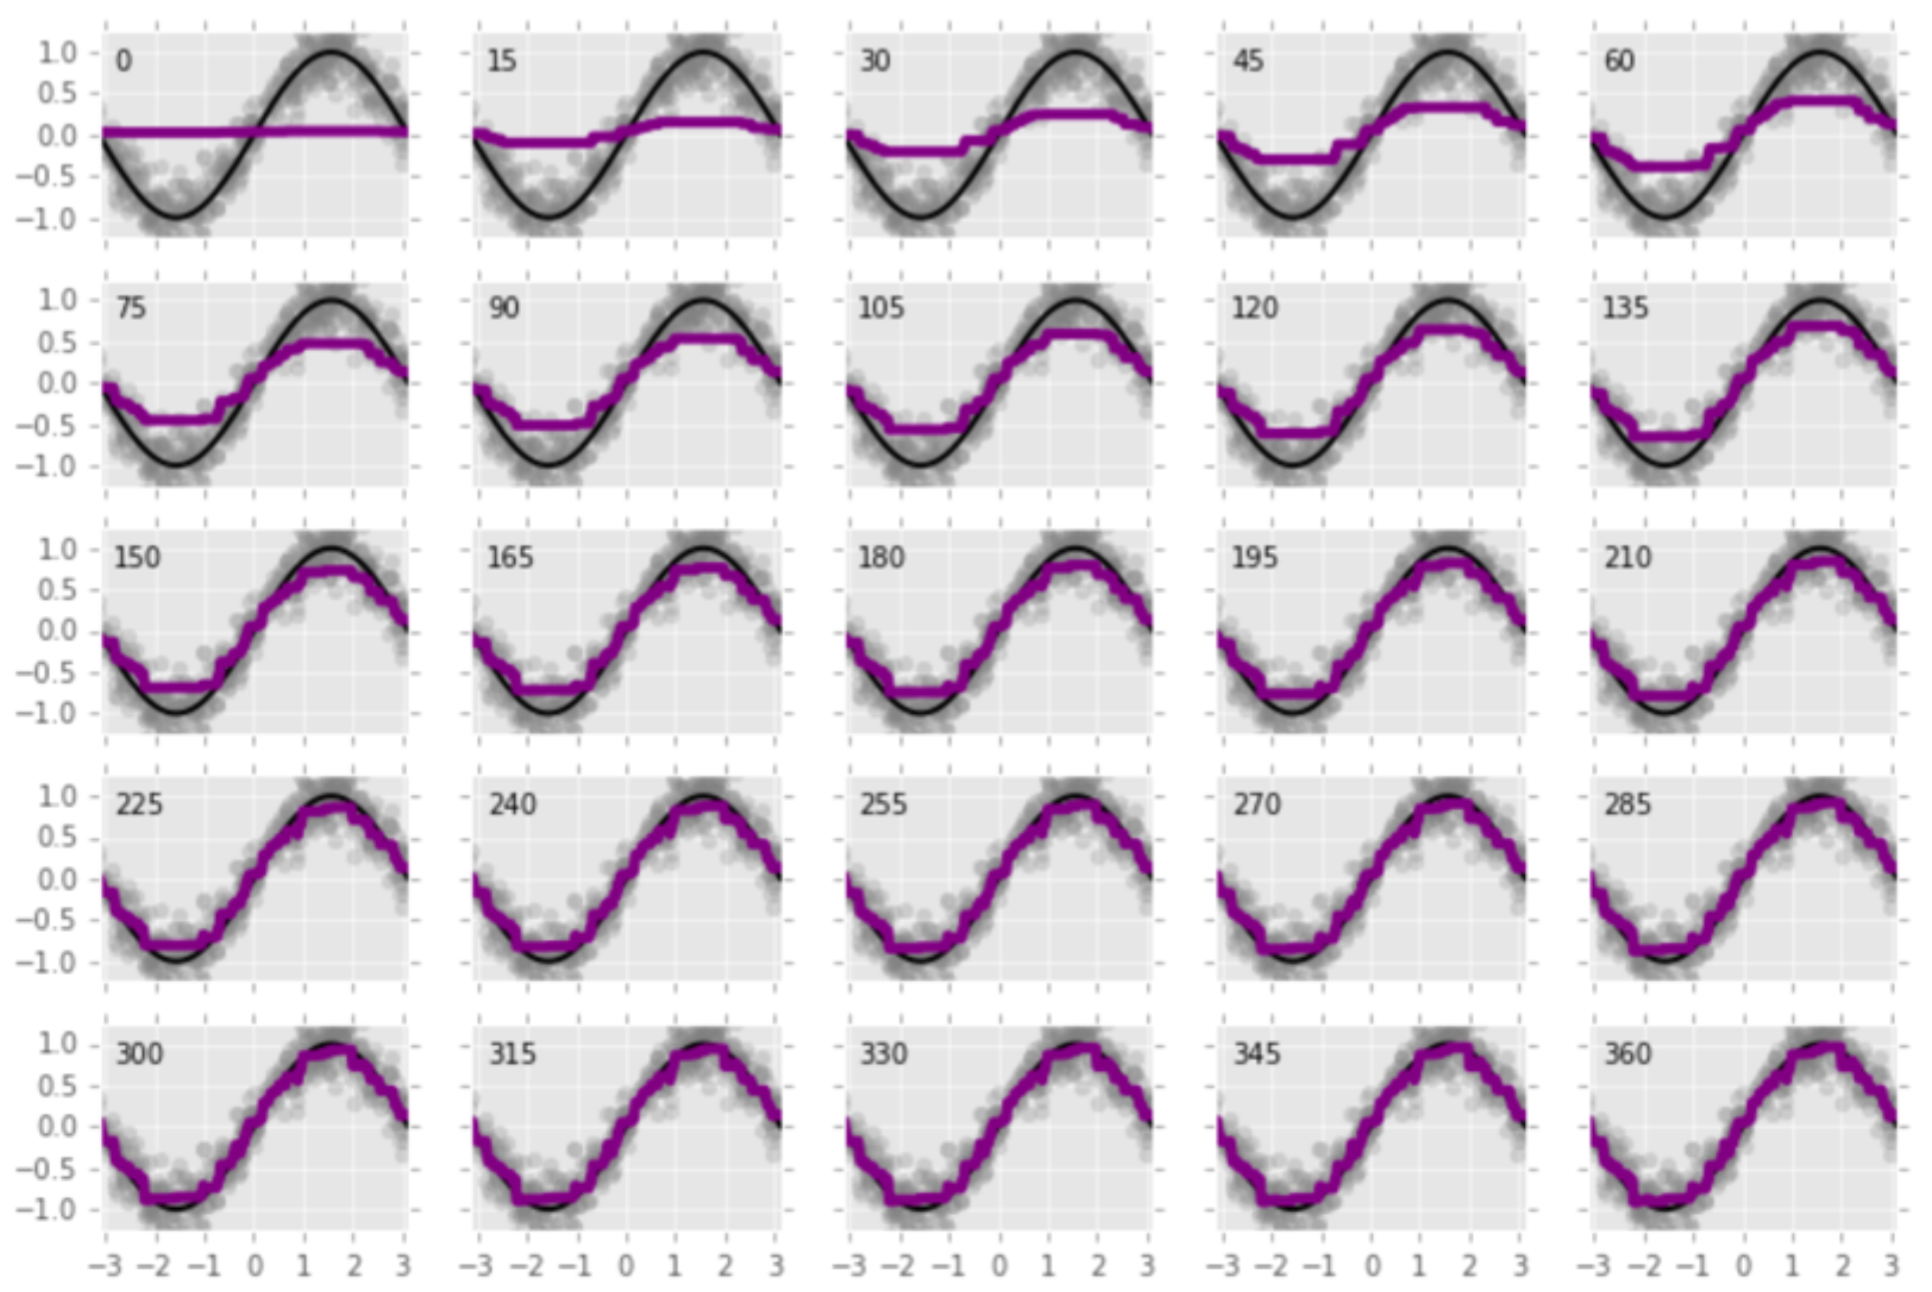
\includegraphics[width=4in]{stuff/boosting4.png}
\end{figure}
}


\frame
{
 \frametitle{Fitting regressions on sequential residuals}

\begin{figure}
\centering
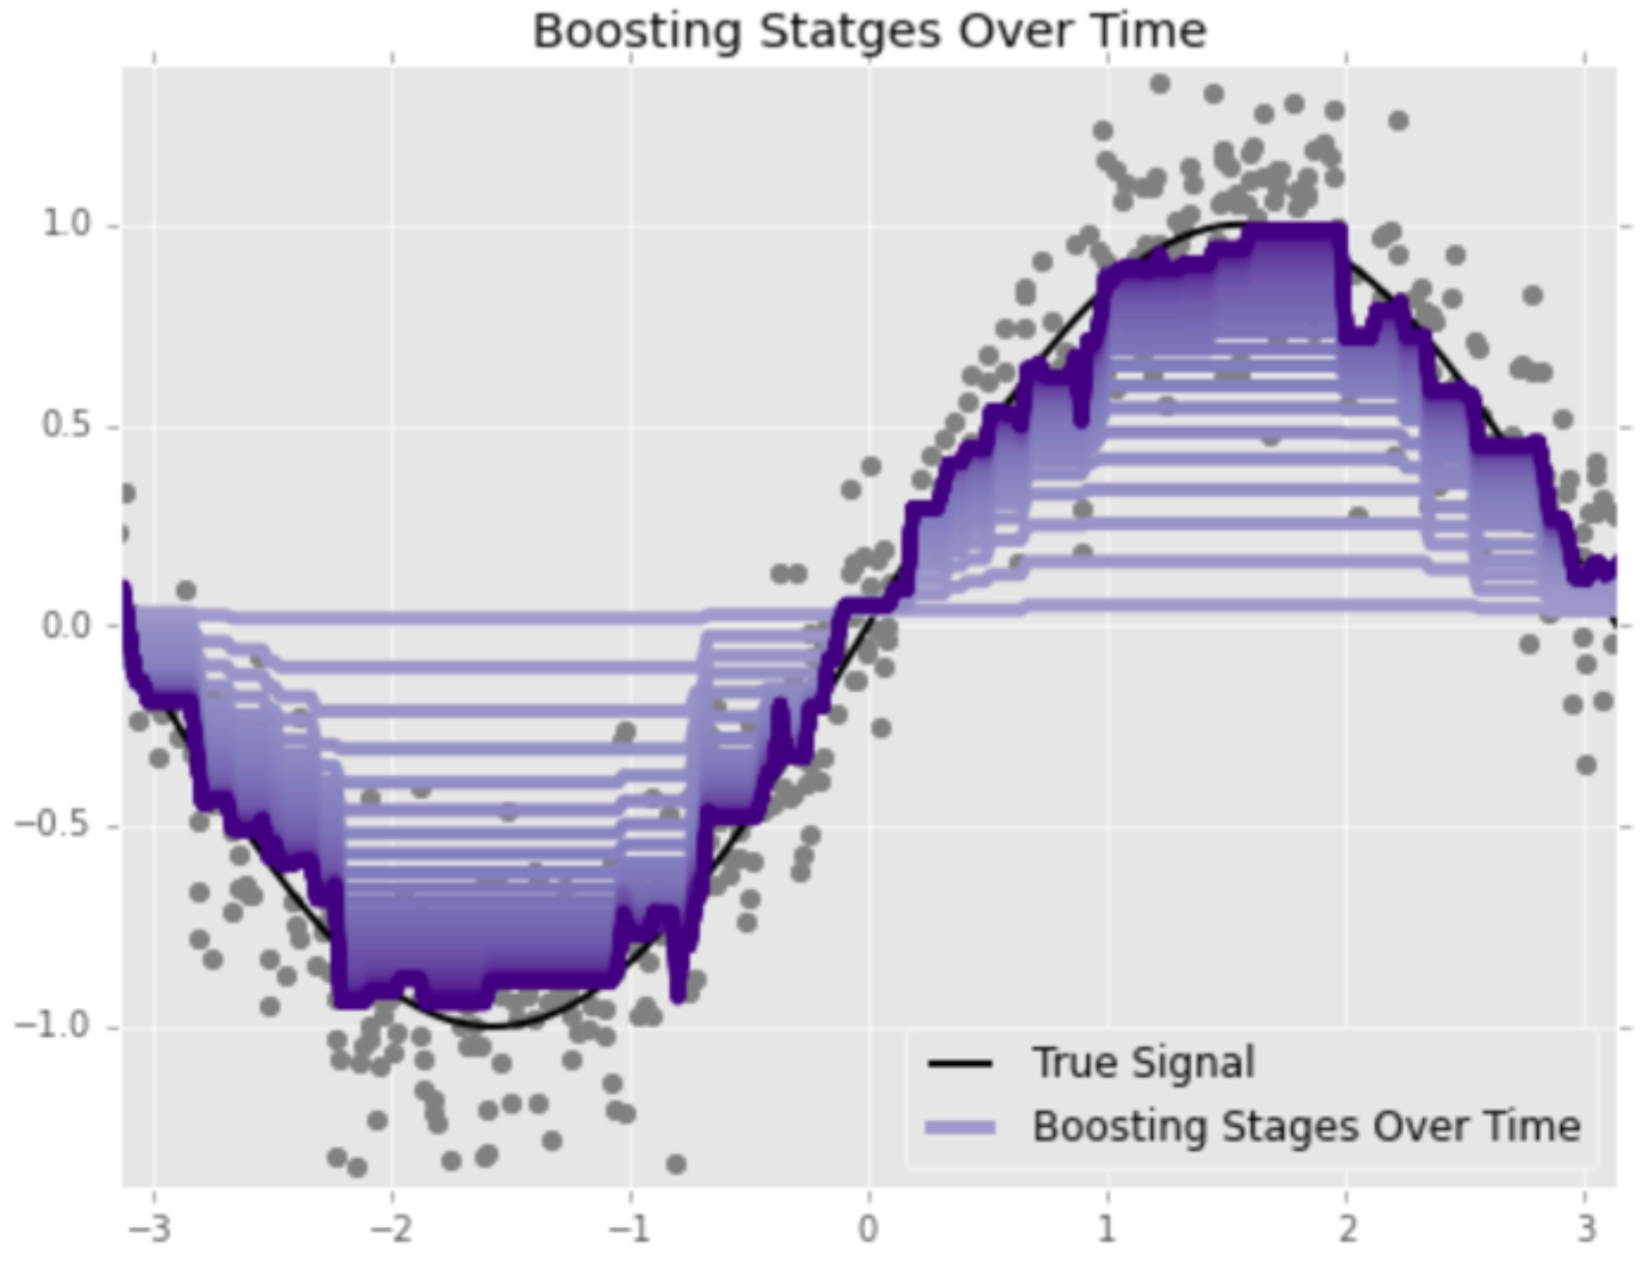
\includegraphics[width=4in]{stuff/boosting5.png}
\end{figure}
}

\frame
{
 \frametitle{Fitting regressions on sequential residuals}

\begin{figure}
\centering
\hspace*{-.375in}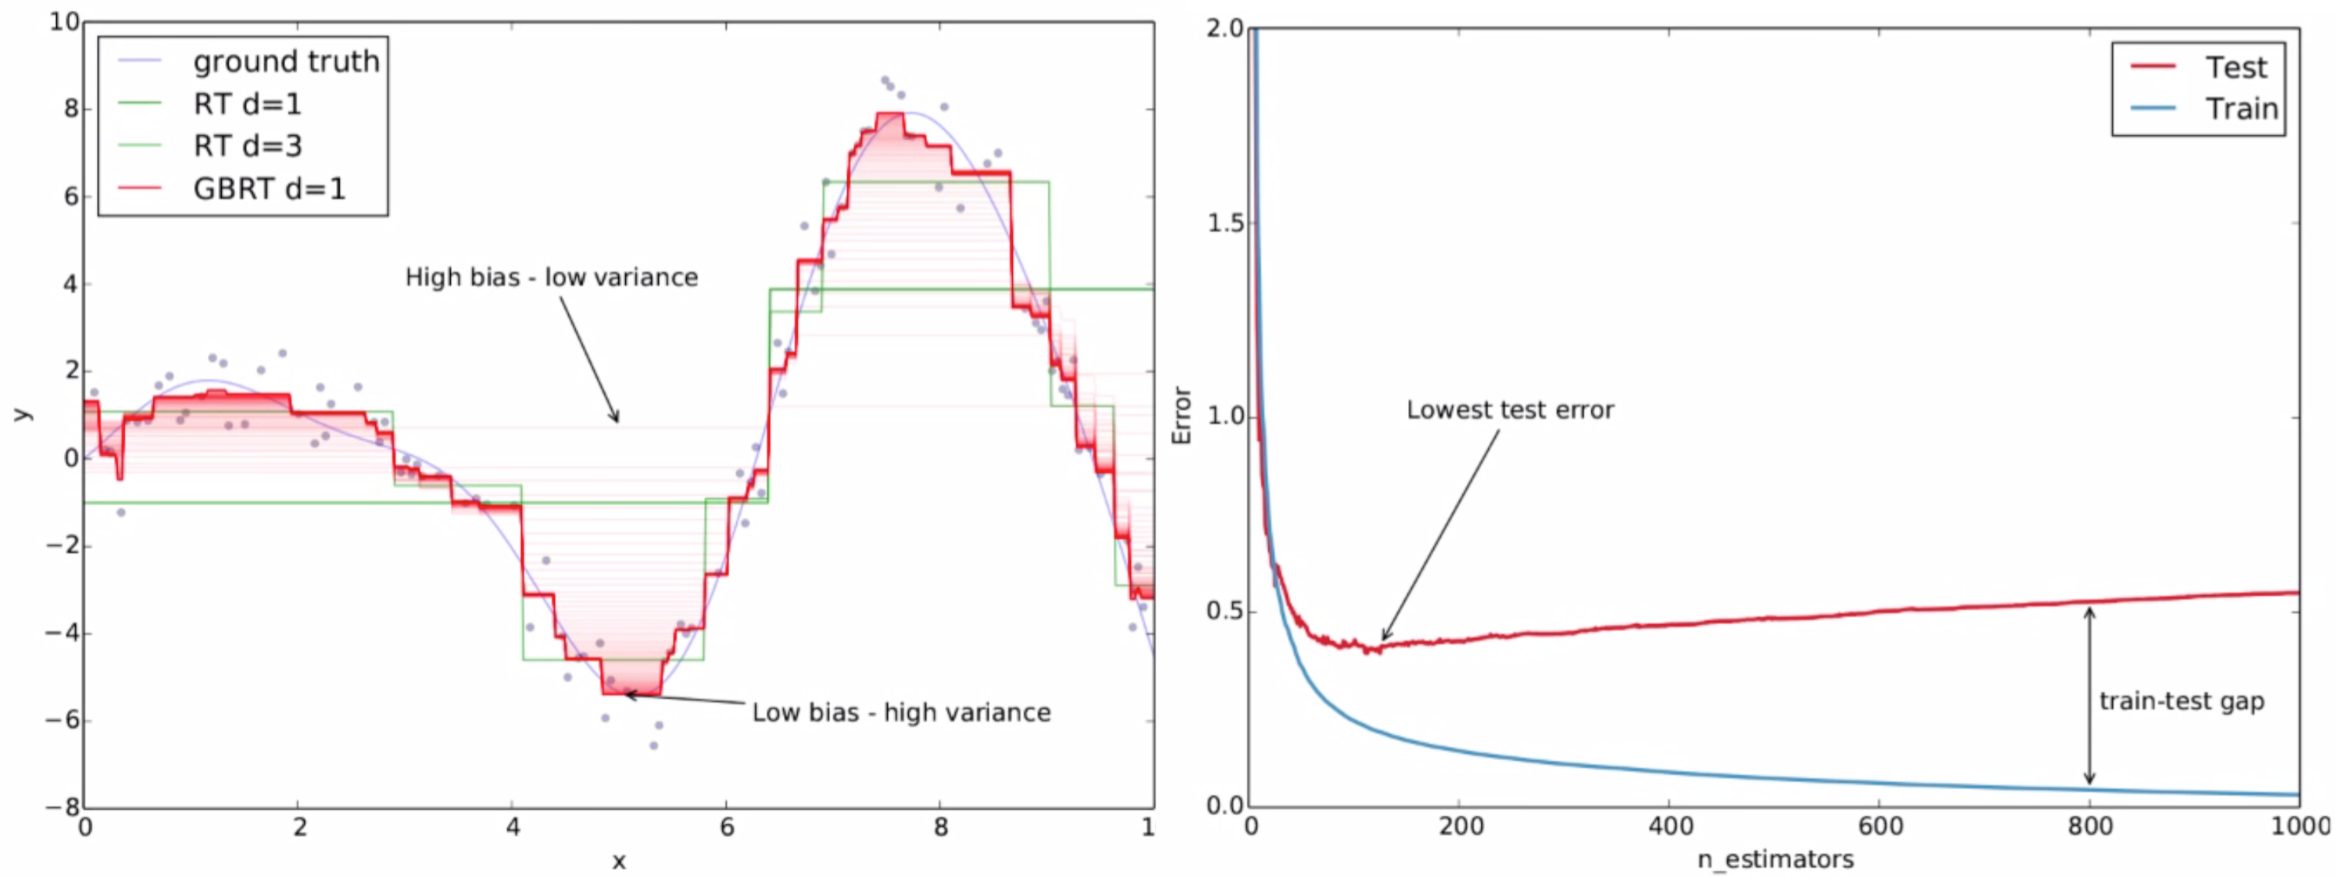
\includegraphics[width=5in]{stuff/boosting3.png}
\end{figure}

\hspace{.45in}\tiny \url{https://www.r-bloggers.com/an-attempt-to-understand-boosting-algorithms/}

}



\frame
{
 \frametitle{Loss Functions}

\begin{itemize}
\item<1-> The \emph{loss function} $L(Y_i, \hat Y_i)$ specifies $\hat Y_i$ prediction (in)accuracy  

\item<2-> \underline{But the prediction $\hat Y_i$ can be changed... \only<3->{oh my...}} 
\item<4-> The gradient of the loss function with respect to $\hat Y_i$ 
$$\frac{\partial L(Y_i, \hat Y_i)}{\partial \hat Y_i}$$

gives the instantaneous $\Delta$ in $L(Y_i, \hat Y_i)$ at  $\hat Y_i \longrightarrow \hat Y_i + \epsilon$
\item[] 
\item[]<5-> \textbf{I.e., it tells how the loss function changes as $\hat Y_i$ increases}
\item[]<5-> \textcolor{gray}{(this is a very simple idea with somewhat complex notation)}

\end{itemize}
}



\frame
{
 \frametitle{Gradient descent}

\begin{itemize}
\item<1-> But if we have partial derivatives we can use gradient descent

\begin{columns}
\begin{column}{.4\textwidth}

$${\nabla}_{\hat {\boldsymbol Y}} L({\boldsymbol Y}, \hat {\boldsymbol Y}) = \left[\begin{array}{c}\frac{\partial L(Y_1, \hat Y_1)}{\partial \hat Y_1}\\
\frac{\partial L(Y_2, \hat Y_2)}{\partial \hat Y_2} \\
\vdots \\
\frac{\partial L(Y_i, \hat Y_i)}{\partial \hat Y_i} \\
\vdots \\
\frac{\partial L(Y_n, \hat Y_i)}{\partial \hat Y_n}\end{array}\right]$$

\end{column}
\begin{column}{.65\textwidth}

\onslide<2->{
\begin{figure}
\centering

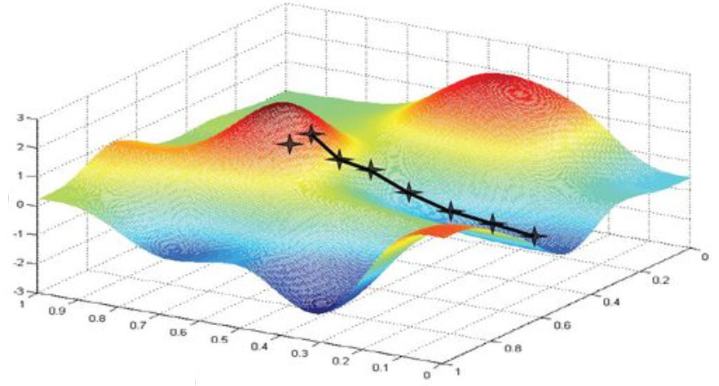
\includegraphics[width=2in]{stuff/gradient.png}
\tiny

The direction of maximal increase is the the gradient of a function\\${}$\\

\textcolor{gray}{\emph{(The negative of the gradient is the direction of maximal decrease)}}

\end{figure}}
\end{column}
\end{columns}

\item[] 
\item[] to move in the direction of greatest decrease in loss  
\end{itemize}
}


\frame
{
 \frametitle{Gradient Boosting}

\begin{itemize}
\item  If we take $\hat Y_i$ to be our current prediction $f_k({\boldsymbol x}_i)$\onslide<2->{, the negative partial derivative of the loss function with respect to $f_k({\boldsymbol x}_i)$
$$\Delta_i^k = -\frac{\partial L(Y_i, f_k({\boldsymbol x}_i))}{\partial f_k({\boldsymbol x}_i)}$$}
\onslide<3->{is the direction of greatest decrease in cost for $\hat Y_i$}
\item<4->[$\Longrightarrow$] \textcolor{red}{We should update $f_k({\boldsymbol x}_i) \rightarrow f_{k+1}({\boldsymbol x}_i)$ in that direction}
\item[]
\item<5-> But $\hat {\boldsymbol Y} = \{\hat Y_1, \hat Y_2, \cdots \hat Y_n\}$ so we compromise between all $\Delta_i^k$ 
$$\hat W(\cdot, \gamma_k) = \underset{W(\cdot, \gamma_k)}{\text{argmin}} \sum_{i=1}^n D(\Delta_i^k, W({\boldsymbol x}_i, \gamma_k)) $$

and set 
$$f_{k+1}({\boldsymbol x}) = f_k({\boldsymbol x}) + \alpha_k \hat W({\boldsymbol x}, \gamma_k)$$ 

\textcolor{gray}{where $\hat W(\cdot, \gamma_k)$ is a \emph{weak learner} boosted at \emph{learning rate} $\alpha_k$} 

\end{itemize}

}


\frame
{
 \frametitle{Fitting regressions on sequential residuals}
\begin{itemize}
\item if we use squared error loss
$$L(Y_i, f_k({\boldsymbol x}_i)) = \frac{1}{2}(Y_i - f_k({\boldsymbol x}_i))^2$$
then the direction of the gradient is vector $ \epsilon_i$ of residuals 
\end{itemize}

\vspace{-2em}
\begin{figure}
\centering
\hspace*{-.75cm}\raisebox{1cm}{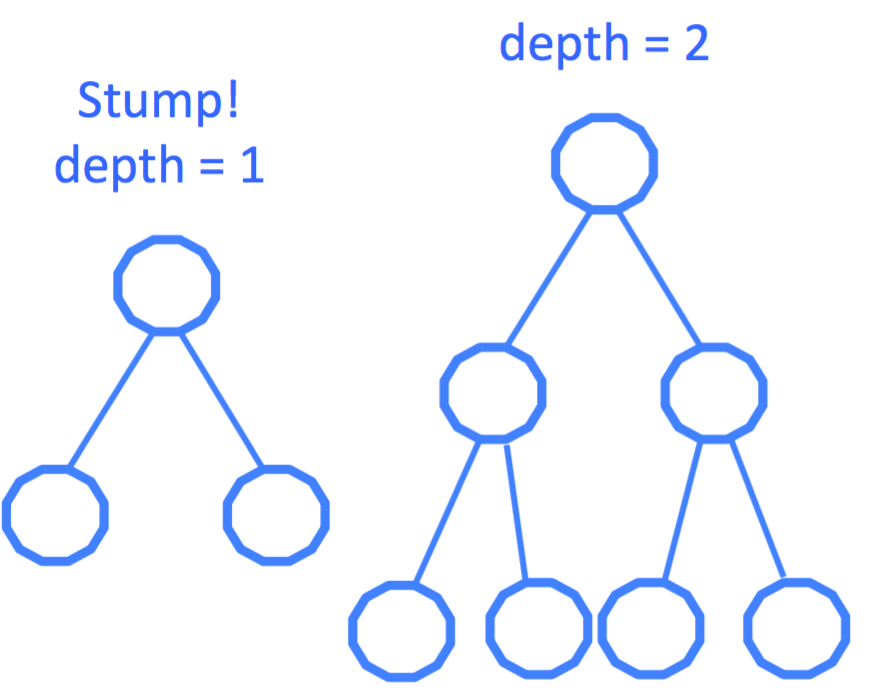
\includegraphics[width=.85in]{stuff/stump.png}}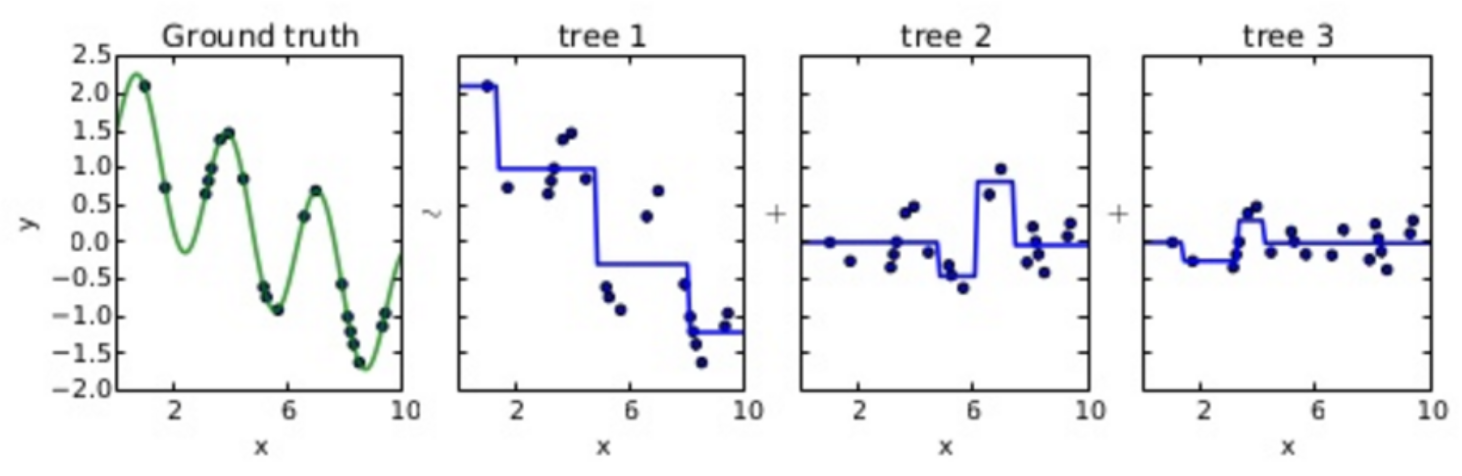
\includegraphics[width=4in]{stuff/residualsgradient.png}
\end{figure}
\vspace{-1.5em}
\begin{itemize}
\item<2-> Moving from $f_k({\boldsymbol x}_i)$ to $f_k({\boldsymbol x}_i) +  \epsilon_i$
 would be zero loss
\item<3-> But we \textbf{don't} move exactly to $f_k({\boldsymbol x}_i) + \epsilon_i$ because
\begin{itemize}
\item<4-> $W({\boldsymbol x}, \gamma_k)$ is a weak learner and probably can't, and
\item<5-> we only move to $f_k({\boldsymbol x}) + \alpha_k \hat W({\boldsymbol x}, \gamma_k)$ at  learning rate $\alpha_k$
\end{itemize}
\end{itemize}

}


\frame
{
 \frametitle{Some loss functions}

\begin{tabular}{rcl}
\underline{Regression}\\
Squared Loss & $\frac{1}{2}(Y_i-{\boldsymbol x}_i^T \boldsymbol\beta)^2$ \\
Absolute Loss & $|Y_i-{\boldsymbol x}_i^T \boldsymbol\beta|$  \\\\
\underline{Classification \{-1, 1\}} \\
Log Loss & $\frac{1}{ln 2} ln(1+e^{-Y_i/\left(1+e^{-{\boldsymbol x}_i^T \boldsymbol\beta}\right)})$ &  (Logistic Reg.) \\
Exponential Loss & $\exp(-Y_i \cdot {\boldsymbol x}_i^T \boldsymbol\beta)$ & (Ada Boost)\\
\end{tabular}

\begin{figure}
\centering
\raisebox{.3em}{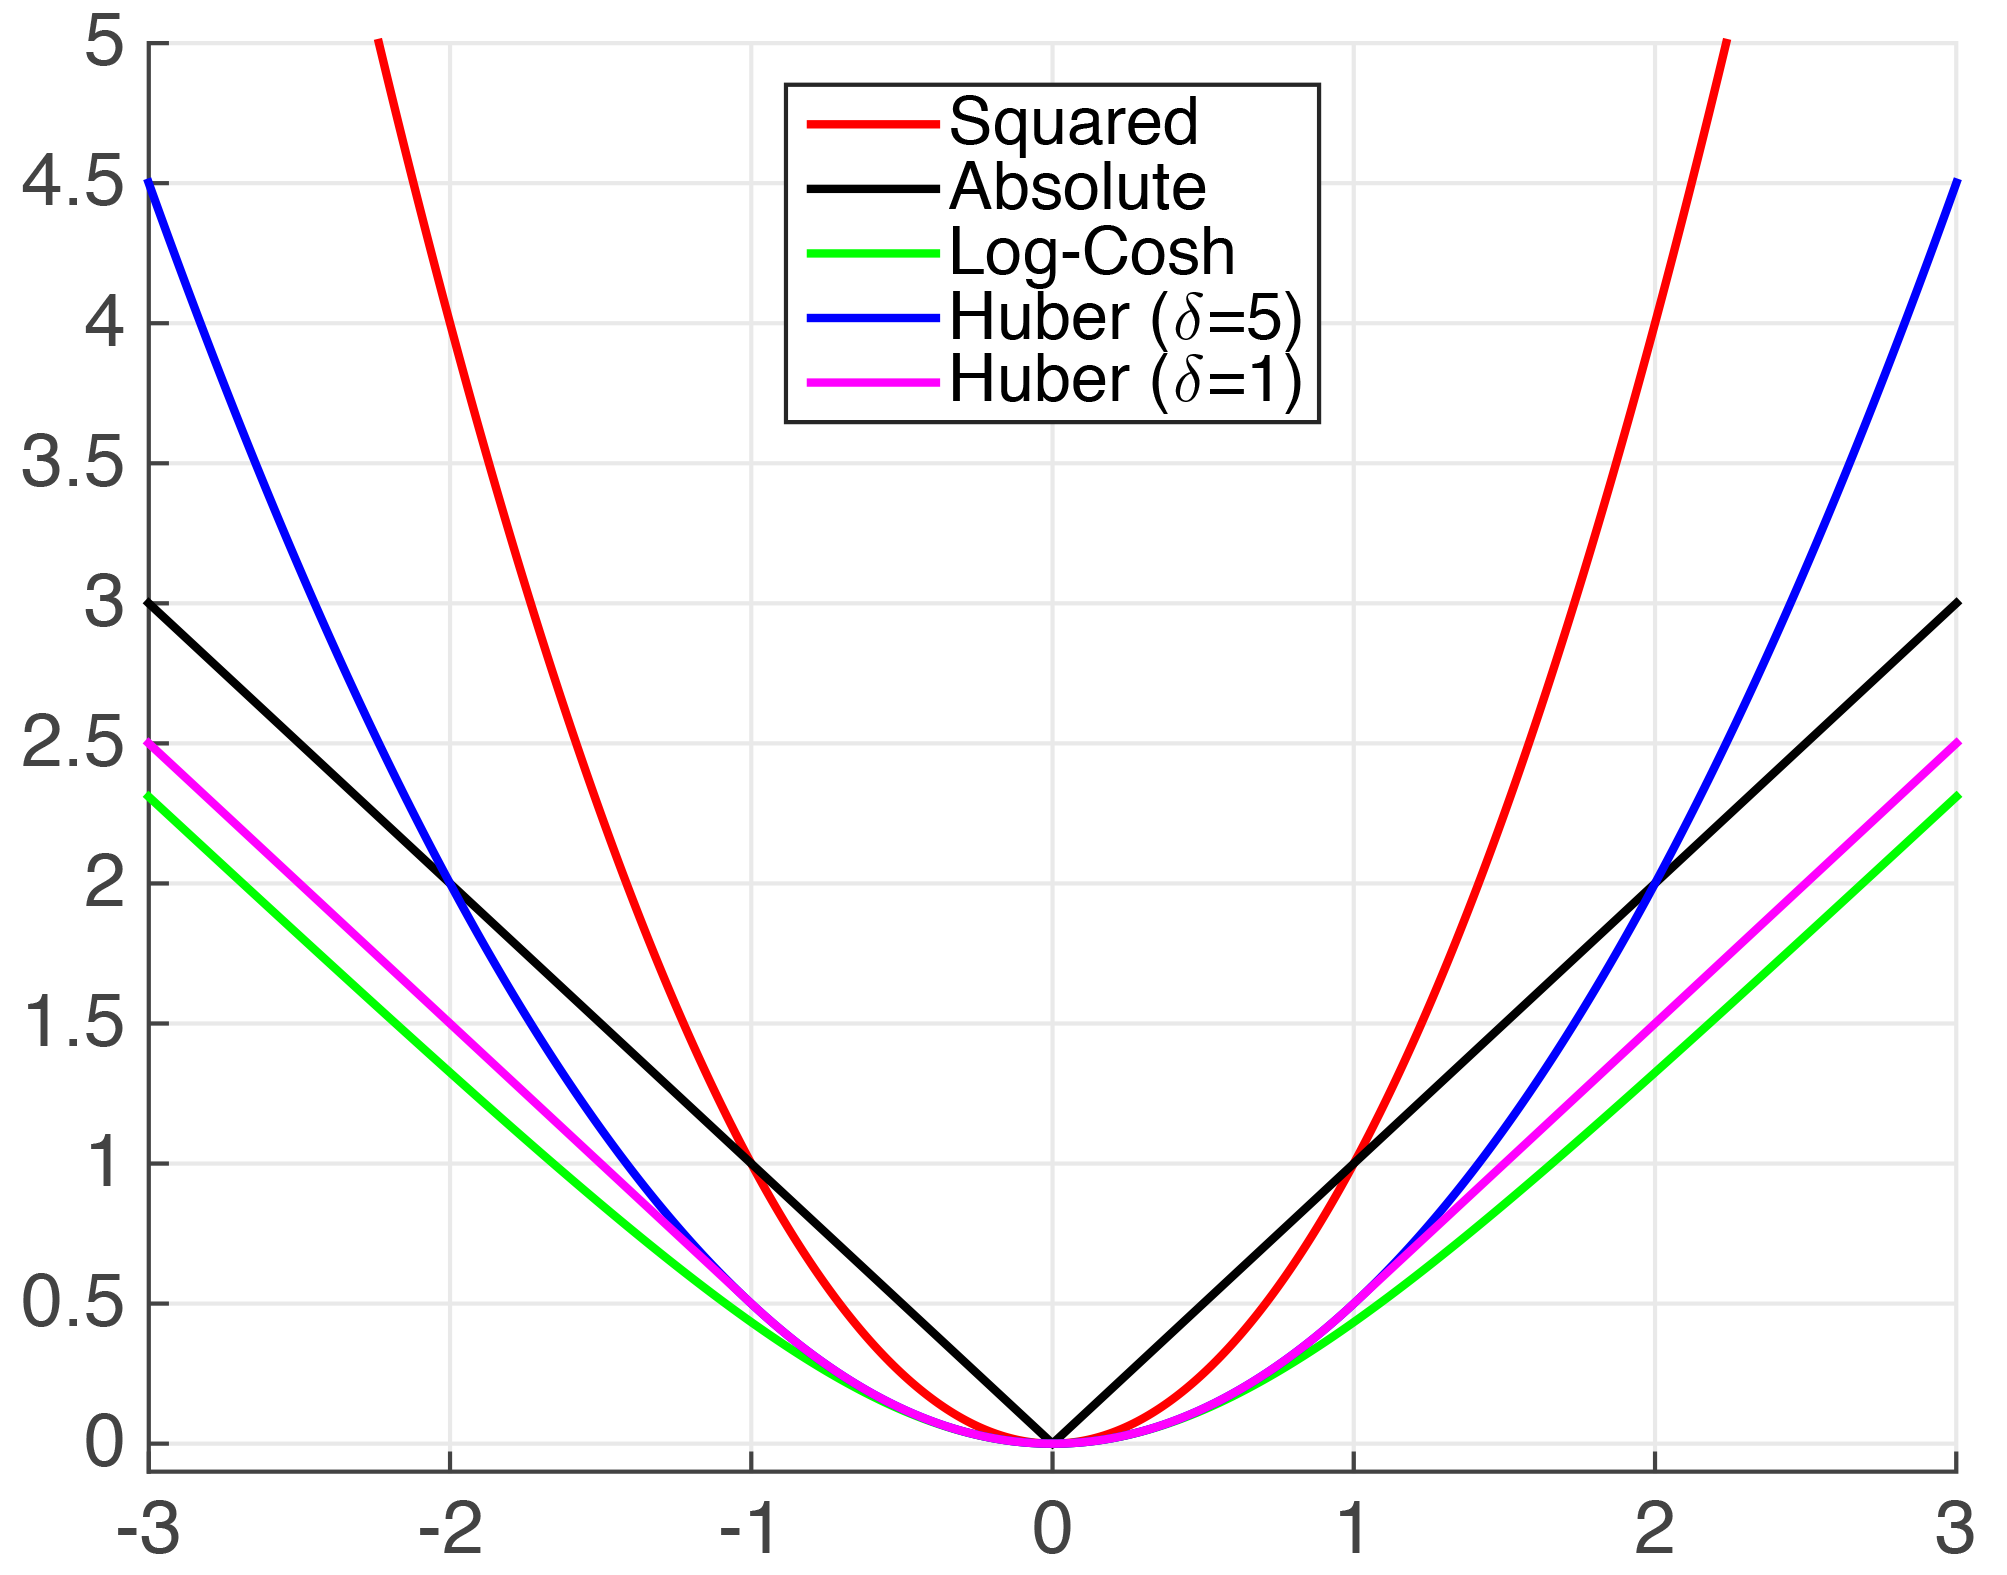
\includegraphics[height=1.5in]{stuff/loss1.png}}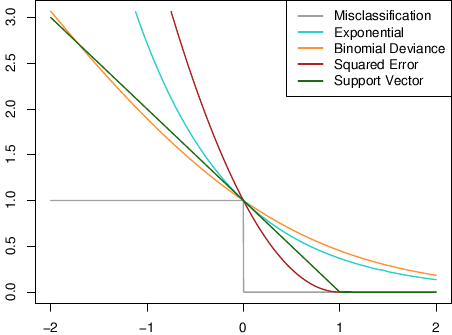
\includegraphics[height=1.5in]{stuff/loss2.png}

\vspace{-1.75em}
$$\;\;{\boldsymbol x}_i^T \boldsymbol\beta \;\quad\quad\quad\quad\quad\quad\quad\quad\quad\quad\quad {\boldsymbol x}_i^T \boldsymbol\beta$$
\end{figure}


}


\frame
{
 \frametitle{Gradient Boosting \textcolor{gray}{VS} Gradient Descent}

\huge

\hspace*{-.75em}$\displaystyle \frac{\partial L(Y_i, \hat Y_i = \boldsymbol x_i^T\boldsymbol \beta)}{\partial \hat Y_i} \text{ \textcolor{gray}{VS} } \frac{\partial L(Y_i, \hat Y_i = \boldsymbol x_i^T\boldsymbol \beta)}{\beta_j}$

}


\frame
{
 \frametitle{AdaBoost (Adaptive Boosting)}
 
\textcolor{gray}{$Y \in \left\{-1,1\right\} \quad$ $W(\cdot,\gamma_k)$ is a ``weak learner''} 
 \begin{enumerate}
 \item Set weights $w^{(1)}_i = \frac{1}{n}$

 \item<2-> For $k = 1, \cdots m$ \\ 
 \begin{enumerate}
\item<3-> Fit $W(\cdot,\gamma_k)$ to the weighted data \textcolor{gray}{using weights $w^{(k)}_i$} 
\item<4-> Compute error $\hat \epsilon_k = \frac{\underset{Y_i \not = W({\boldsymbol x}_i,\gamma_k)}{\sum} w^{(k)}_i }{\sum w^{(k)}_i}$ 
\item<5-> Compute $\alpha_k = log\left(\frac{1}{\hat \epsilon_k} - 1\right)$
\item<6-> Set $w_i^{(k+1)} = w_i^{(k)} e^{\alpha_k 1_{[Y_i \not = W({\boldsymbol x}_i,\gamma_k)]}}$
\end{enumerate}
\item<7-> Return $G({\boldsymbol x}_i) = \text{sign}\left(\sum_{k=1}^m \alpha_k W({\boldsymbol x}_i,\gamma_k)\right)$ 
\end{enumerate}
 
\begin{figure}
\centering
\onslide<8->{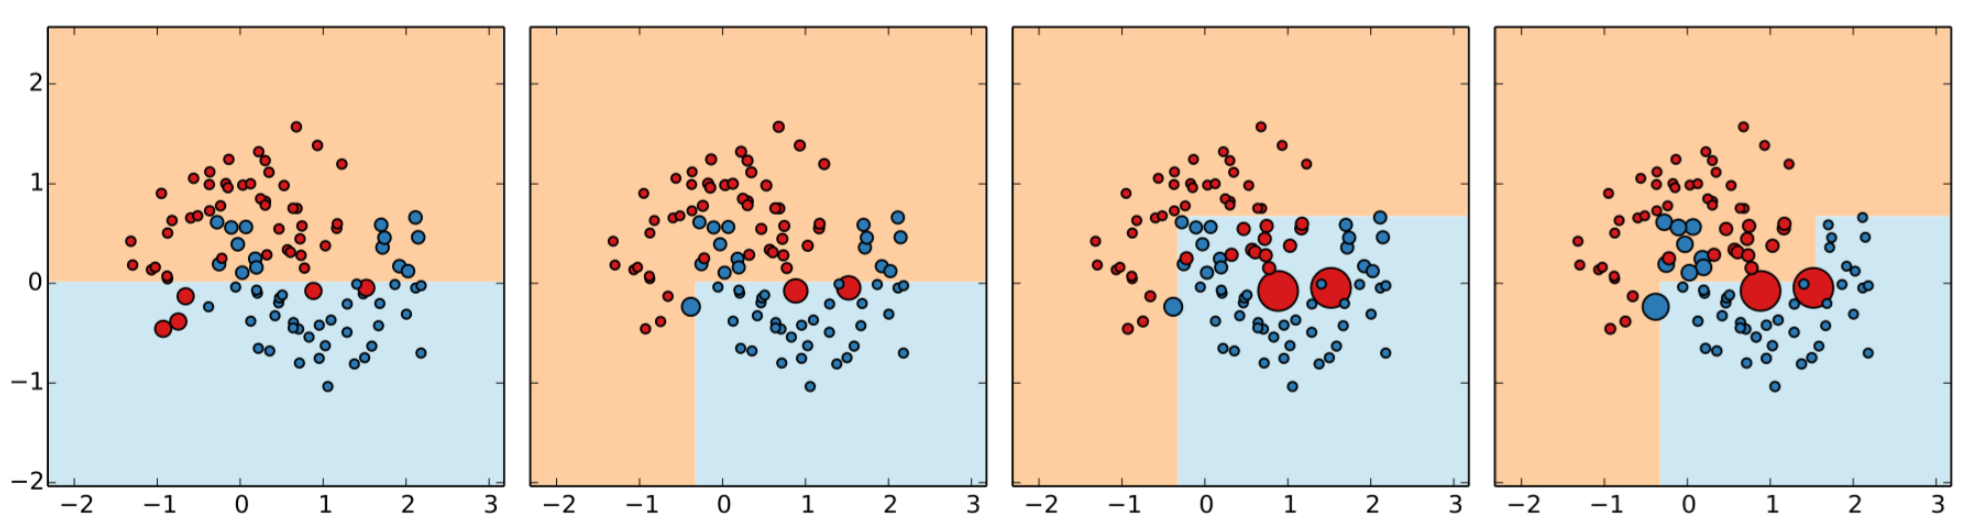
\includegraphics[width=4in]{stuff/adaboost1.png}}\\
\onslide<9->{\scriptsize *Sean Sall's slides have an appendix showing that AdaBoost is exponential loss}
\end{figure}
 
}

\frame
{
 \frametitle{XGBoost (eXtreme Gradient Boosting)}

\begin{itemize}
\item Percentiles binned features: faster/more efficient splitting 
\item Handles missing data
%\item Handles mixed data types
\item Smart memory management/out-of-core computation\\
$\quad\quad\quad\quad\quad\quad\quad\quad\quad$\textcolor{gray}{(i.e., data too big to fit into memory)}
\item[] 
\end{itemize}

\url{http://xgboost.readthedocs.io}
\begin{itemize}
\item Knobs
\item Get Started (Python Install)
\item Packages $>$ Python $>$ Python API Reference
\begin{itemize}
\item Core Data Structure
\item Learning API
\item Scikit-Learn API
\end{itemize}
\end{itemize}

}



\frame
{
\frametitle{New Segment: ``Scott's Sage Words of Wizdum''}

\tiny 
\begin{itemize}
\item If your ``in sample'' prediction error matches your ``out of sample'' prediction error, your model is generalizing well out of sample.
\item Otherwise, you're overfitting. 
\item This is checked with K-folds cross-validation.
\item If you're generalizing well out of sample, then you might as well use all your data for your final fit.
\item If you're not then generalizing well out of sample (or even if you are) you can get a feel for the types of errors you'll make (based on your prediction performance from K-folds); you can aggregate your fits across the K-folds somehow and expect that sort of error.  
\item Aggregating and using all your data when you know you're overfitting means you know you have overfitting issues (and kind of know what they are based on k-folds) but you're happy to use all your data and risk even further overfitting anyway.  LOO cross validation might be a reasonable way to assess what your actual errors would be under the ``full data usage'' approach. 
\item[] 
\item Random Forests \emph{can} overfit; but not because you add more trees; rather, because the trees can be very complex (though this can be tuned) and therefore fit idiosyncrasies of the data (even in spite of the bootstrapping -- i.e., the idiosyncrasies that still show through in the bootstrapping). 
\item Random Forests just don't overfit as a result of adding more predictors (i.e., trees).
\item OOB and training error \emph{are not} the same thing; yes, OOB tells you how you generalize \emph{within your training set}, but that doesn't matter if your test set has associations that are not reflected in the training set. 
\item This is of course also the same risk in K-folds... but, as with OOB, one hopes such problems aren't present
\item Or, all of these methods can overfit (find spurious associations or chase outliers) in sample.  OOB doesn't save you from that.  And of course OOB is not apples to apples  across methodologies. 
\item[]
\item Random forests are built in a very structured, data partitioning manner that can have some intrinsic bias, actually.  Because boosting moves so slowly, sequentially rather than instantaneously partitioning the data, it can remove that bias.  And while too many trees can cause boosting to be a high variance (overfitting prone) model, boosting moves so slowly that actually it is not so responsive to outlier data points until deep into the process.
\item[]
\item all of these methods can overfit in sample but still potentially improve in out of sample performance
over models that are capturing more ``generalizable'', but coarser, associations.  
\item Inference here may not be key for prediction then, unless of course extrapolations are needed and work under the simpler model
\item Inference is needed when you don't have the ability to perform predictive testing
\end{itemize}


}



\end{document}
% NP
% model grows with data
% prediction are based on parameter/coefficient estimates
% parameters are estimated and these define an instance of a class
